%\documentclass[12pt]{article}
%\usepackage[a4paper, margin=1in]{geometry} 
%\usepackage{graphicx} 
%\usepackage{hyperref}
%\usepackage{float}
%\usepackage{multicol}
%\usepackage{multirow}
%\usepackage{amsmath}
%\usepackage[font=small, labelfont=bf]{caption}
%
%\begin{document}

%
% Viterbi algorithm
%
\subsection{Viterbi algorithm}
The Viterbi algorithm is used to find the most probable path of HMM.

%
% Probabilities of possible paths when the states are unknown
%
\subsubsection*{Probabilities of possible paths when the states are unknown}
All possible paths need to be considered for an observed instance when the states are unknown. 

%
% Example of all possible paths
%
\subsubsection*{Example of all possible paths}
How many possible paths can one find when there are two states \{S1, S2\} and three observation \{O1, O2, O3\}? \\

\noindent
The number of all possible paths: 8 \\
(S1, S1, S1), (S1, S1, S2), (S1, S2, S1), (S1, S2, S2), \\
(S2, S1, S1), (S2, S1, S2), (S2, S2, S1), (S2, S2, S2)

%
% Dynamic programming
%
\subsubsection*{Dynamic programming}
The Viterbi algorithm is a dynamic programming that can be used to find the most probable path and its probability of an HMM.

%
% Example of dynamic programming
%
\subsubsection*{Example of dynamic programming}
\begin{figure}[H]
  \centering
      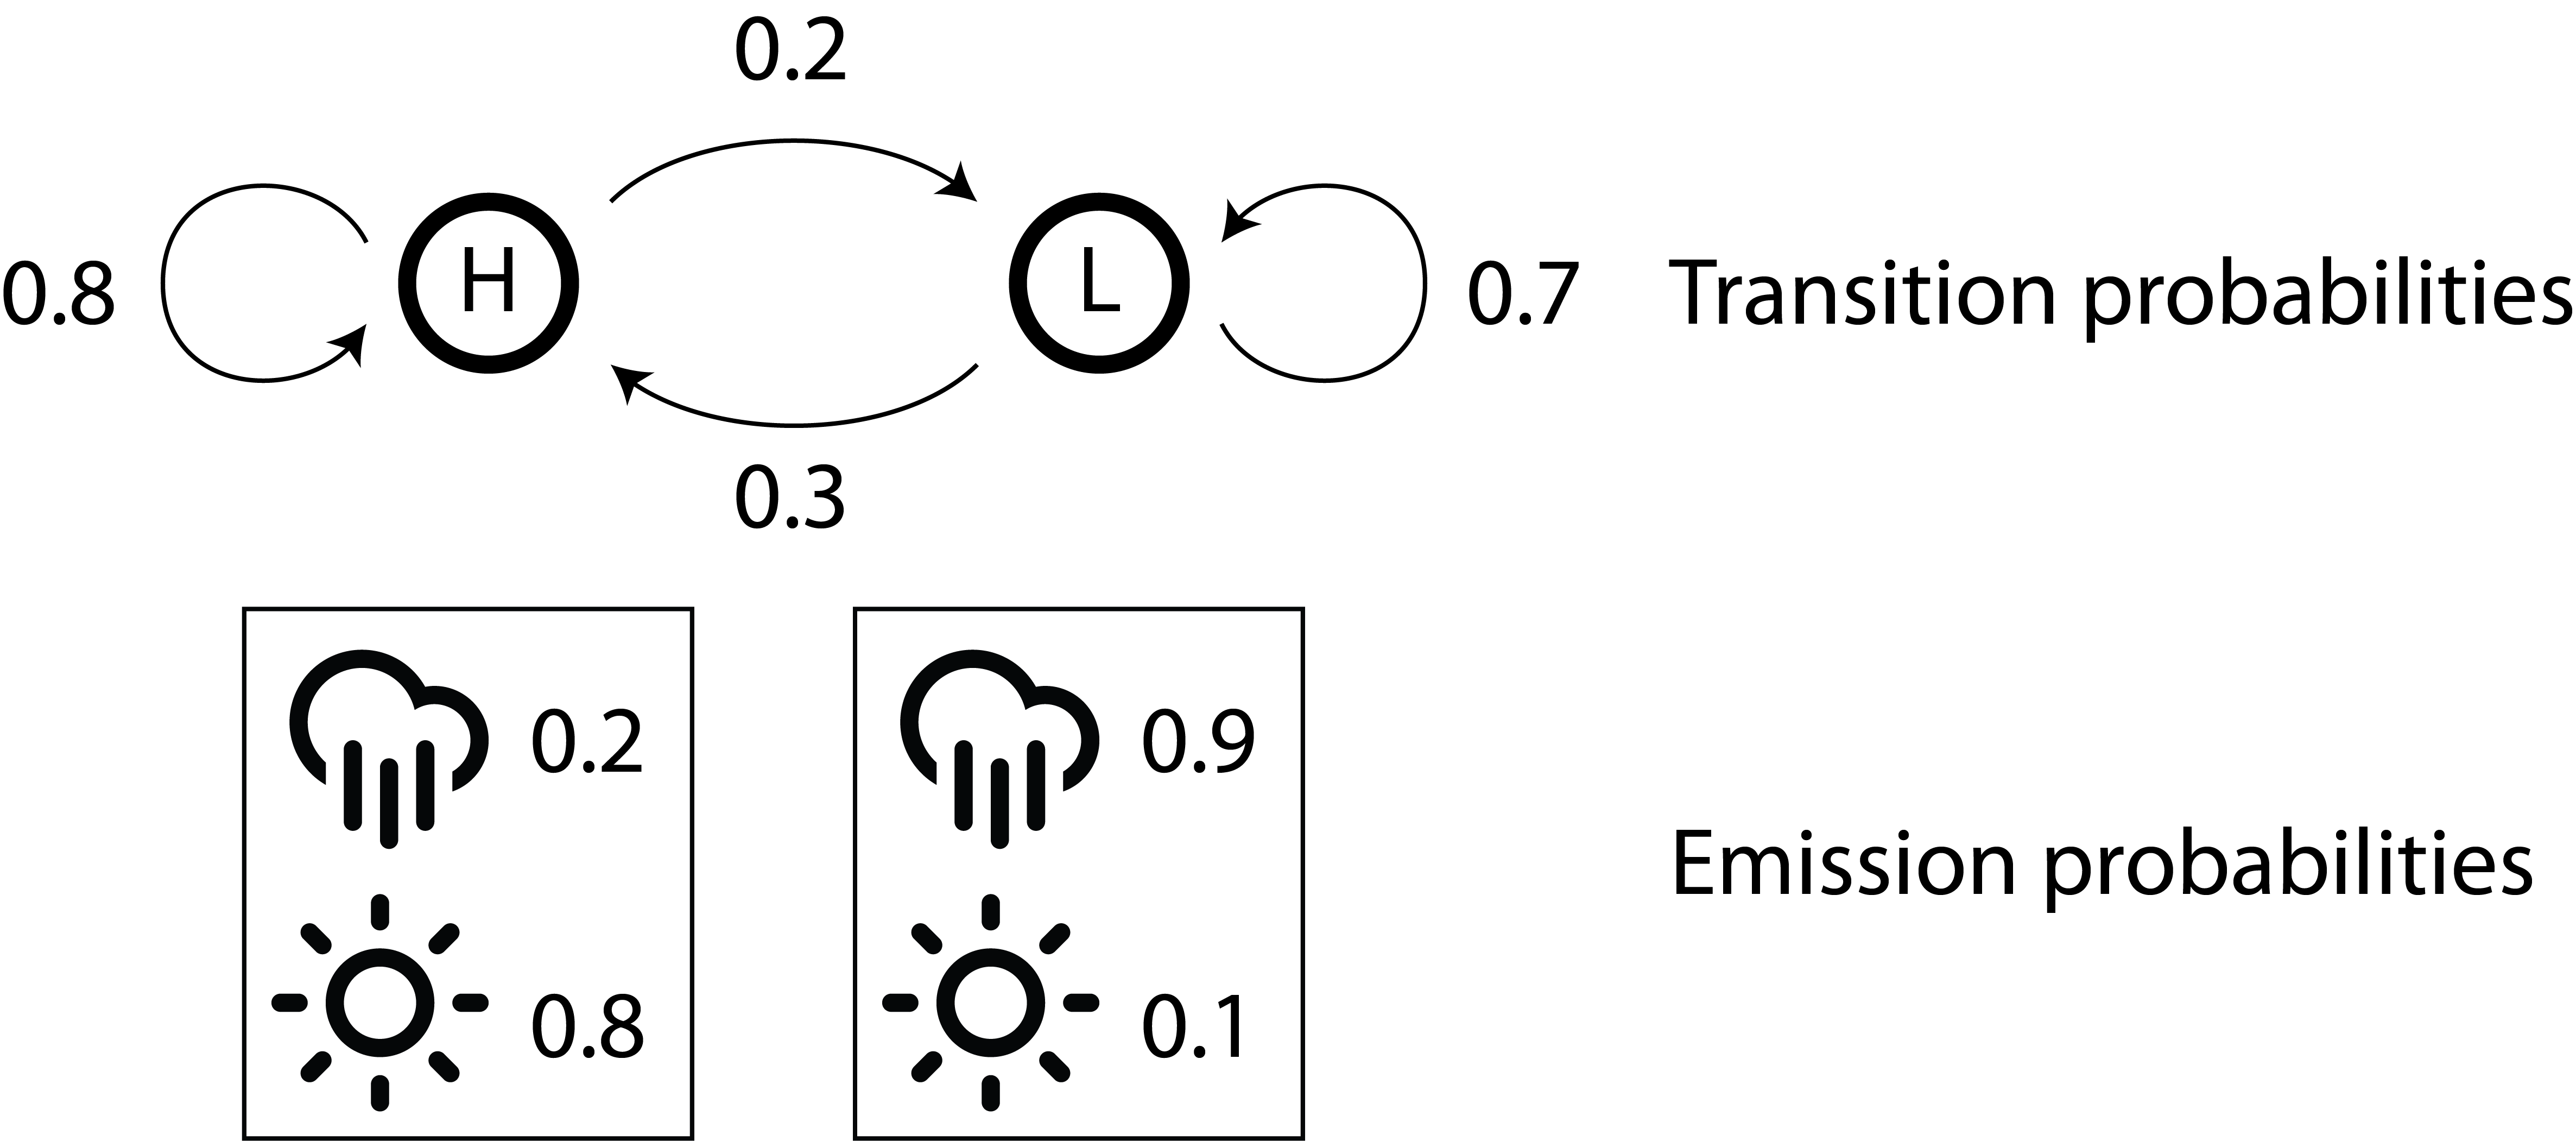
\includegraphics[width=0.5 \textwidth]{fig13/HMM_example.png}
  \caption{HMM for weather conditions}
\end{figure}

Find the most probable path in the HMM above when the observed weather conditions are (Sunny, Sunny, Sunny). Assume no particular prior distribution for the initial states.

\begin{table}[H]
\centering
\caption{DP table for the Viterbi algorithm}
\label{my-label}
\begin{tabular}{|c|l|l|}
\hline
                       & \multicolumn{1}{c|}{H}     & \multicolumn{1}{c|}{L}     \\ \hline
Sunny                  & $0.5 \times 0.8 = \textbf{0.4}$              & $0.5 \times 0.4 = 0.2$              \\ \hline
\multirow{2}{*}{Sunny} & (H)$0.4 \times 0.8 \times 0.8 = \textbf{0.256}$     & (H)$0.4 \times 0.2 \times 0.1 = 0.008$     \\
                       & (L)$0.2 \times 0.3 \times 0.8 = 0.048$     & (L)$0.2 \times 0.7 \times 0.1 = 0.014$     \\ \hline
\multirow{2}{*}{Sunny} & (H)$0.256 \times 0.8 \times 0.8 = \textbf{0.16384}$ & (H)$0.256 \times 0.2 \times 0.1= 0.00512$  \\
                       & (L)$0.014 \times 0.3 \times 0.8 = 0.00336$ & (L)$0.014 \times 0.7 \times 0.1 = 0.00098$ \\ \hline
\end{tabular}
\end{table}

%
% Exercise \thesection.2
%
\subsubsection*{Exercise \thesection.2}
Use the the HMM above and find the most probable path for the following weather conditions. Assume no particular prior distribution for the initial states.

\begin{enumerate}
\item (Sunny, Rain).
\begin{table}[H]
\centering
\begin{tabular}{|c|c|c|}
\hline
      & H & L \\ \hline
Sunny & \quad \quad \quad \quad  \quad \quad \quad \quad &  \quad \quad \quad \quad \quad \quad \quad \quad \\ \hline
Rain  &   &    \\ \hline
\end{tabular}
\end{table}

\item (Rain, Rain).
\begin{table}[H]
\centering
\begin{tabular}{|c|c|c|}
\hline
      & H & L \\ \hline
Rain & \quad \quad \quad \quad  \quad \quad \quad \quad &  \quad \quad \quad \quad \quad \quad \quad \quad \\ \hline
Rain  &   &    \\ \hline
\end{tabular}
\end{table}

\end{enumerate}

\bigskip 

%\end{document}
